% !TeX program = lualatex
% !TeX encoding = utf8
% !TeX spellcheck = uk_Ua

\documentclass[
    10pt,
    % handout % Remove all incremental effects (<+->) and display all bullet points at once.
]{beamer}
\usepackage{fontspec}
\setsansfont{Arial}

\usepackage[english, ukrainian]{babel}

\usepackage{graphicx}
\usepackage{wrapfig}
\usepackage{float}
\usepackage{color}

\setbeamercovered{transparent}
\usetheme{Boadilla}
\usecolortheme{seahorse}

\author{КМ-11 Омельченко Іван}
\title{Бакалаврська кваліфікаційна робота}
\date{21.05.2025}

\setbeamercolor{block title}{bg=blue!20, fg=black}

% видаляємо навігаційну панель
\makeatletter
\setbeamertemplate{navigation symbols}{}

\usepackage{tabularray}
\usepackage{mathtools,amsfonts,amsthm}
\usepackage{xurl}

\usepackage{tikz}
\usetikzlibrary{arrows.meta}
\usepackage{pgfplots}
\usepackage{pgfplotstable}
\pgfplotsset{compat=newest}

\usepackage{float}
\usepackage{microtype}
\usepackage{cmap}
\usepackage{xcolor}

\begin{document}

%%% --------------------------------------------------------------------
\section{Титульна сторінка}
%%% --------------------------------------------------------------------

\begin{frame}
    \begin{center}
        \textbf{\Large Дипломна робота}
    \end{center}

    \begin{block}{}
        \centering\Large
        \vspace{1mm}
        Адаптивний шаховий бот на основі глибинного навчання
        \vspace{2mm}
    \end{block}

    \vspace{0.7cm}

    \begin{columns}
        \begin{column}{0.65\textwidth}
            \small
            \textbf{Виконав:} студент IV курсу, КМ-11 \\
            Омельченко Іван \\ \vspace{2mm}
            \textbf{Науковий керівник:} \\
            завідувач кафедри ПМА, канд. техн. наук, доцент \\ 
            Тавров Данило Юрійович
        \end{column}

        \begin{column}{0.35\textwidth}
            \vspace{0.1cm}
            \begin{center}
                
\includegraphics[width=0.95\linewidth]{Images/student_id.png}
            \end{center}
        \end{column}
    \end{columns}
\end{frame}


%%% --------------------------------------------------------------------
\section{Постановка задачі}
%%% --------------------------------------------------------------------

\newcounter{subtopic}

\stepcounter{subtopic}
\begin{frame}[t]
    \frametitle{\insertsection}
    \begin{itemize}
        \item Сучасні шахові рушії (Stockfish, Lc0) демонструють надлюдську силу, але не імітують людське мислення.
        \item Їхні ходи часто неприродні для гравців, що ускладнює навчання та аналіз.
        \item Потрібні моделі, які грають \textit{як люди}: з інтуїцією, помилками, стратегічною поведінкою.
        \item Такі рушії мають застосування в освіті, дослідженнях і розвагах.
        \item \textbf{Мета роботи:} створення адаптивного шаховий бота, що відтворює особливості людського стилю гри шляхом глибинного навчання на історичних партіях людей.
        \item \textbf{Кінцевий результат:} шаховий бот із графічним інтерфейсом, що відтворює людський стиль гри на основі історичних партій.
    \end{itemize}
\end{frame}


%%% --------------------------------------------------------------------
\section{Підходи до побудови шахових рушіїв}
%%% --------------------------------------------------------------------

\stepcounter{subtopic}

\begin{frame}[t]
    \frametitle{Класичні шахові рушії}

    \begin{itemize}
        \item \textbf{Приклади:} Stockfish, Komodo, Fritz (3500 Elo).
        
        \item \textbf{Алгоритми пошуку:}
        \begin{itemize}
            \item Мінімакс — знаходить найкращий хід за умови оптимальної гри суперника:
            \item Альфа-бета відсікання — оптимізація, що скорочує кількість розглянутих варіантів без втрати точності.
            \item Результативність залежить від порядку перебору ходів.
        \end{itemize}

        \item \textbf{Евристики оцінки позиції:}
        \begin{itemize}
            \item Матеріальні коефіцієнти (ферзь = 9, тура = 5 тощо).
            \item Позиційні таблиці: активність фігур, контроль центру, структура пішаків.
            \item Поділ на фазу миттельшпілю та ендшпілю.
        \end{itemize}

        \item \textbf{Особливості:}
        \begin{itemize}
            \item Силу гри можна регулювати — зменшуючи глибину пошуку або обмежуючи час на хід.
            \item Проте така регуляція не наближає стиль гри до людського — ходи залишаються неприродними.
        \end{itemize}
    \end{itemize}
\end{frame}

\stepcounter{subtopic}
\begin{frame}[t]
    \frametitle{Класичні рушії: переваги та недоліки}
    \begin{block}{Переваги}
        \begin{itemize}
            \item Дуже сильна гра — краща за будь-яку людину.
            \item Ефективний пошук завдяки альфа-бета відсіченню.
        \end{itemize}
    \end{block}

    \begin{block}{Недоліки}
        \begin{itemize}
            \item Залежність від евристик, створених вручну.
            \item Наявність артифактів адаптувані до рівня суперника (зменшення глибину пошуку).
        \end{itemize}
    \end{block}
\end{frame}

%%% --------------------------------------------------------------------
\section{Нейромережеві шахові рушії}
%%% --------------------------------------------------------------------

\stepcounter{subtopic}
\begin{frame}[t]
    \frametitle{Нейромережеві шахові рушії}

    \begin{itemize}
        \item \textbf{Приклади:} AlphaZero, Leela Chess Zero (Lc0) (3450 Elo).

        \item \textbf{Принцип роботи:}
        \begin{itemize}
            \item Поєднання нейронної мережі з пошуком Monte Carlo Tree Search (MCTS).
            \item Пошук не симулює гру до кінця — мережа використовується для оцінки й вибору ходів.
        \end{itemize}

        \item \textbf{Структура мережі:}
        \begin{itemize}
            \item {Policy (ймовірнісний розподіл ходів):} \(\pi(a \mid s) = P(s, a)\)
            \item {Value (оцінка позиції):} \(v(s) \in [-1, 1]\)
        \end{itemize}

        \item \textbf{Вибір ходу:}
        \begin{itemize}
            \item Використовується формула PUCT:
            \[
                \text{PUCT}(s, a) = Q(s, a) + c_{\text{puct}} \cdot P(s, a) \cdot \frac{\sqrt{N(s)}}{1 + N(s, a)}
            \]
            \item де \(Q(s, a)\) — середнє значення value-оцінки, \(N(s, a)\) — кількість симуляцій, \(P(s, a)\) — policy-пріоритет.
        \end{itemize}

        \item \textbf{Особливості:}
        \begin{itemize}
            \item Оцінка позицій не базується на фіксованих евристиках — її виконує нейромережа, навчена за допомогою методів навчання з підкріпленням.
        \end{itemize}
    \end{itemize}
\end{frame}

\stepcounter{subtopic}
\begin{frame}[t]
    \frametitle{Переваги і недоліки нейромережевих рушіїв}
    \begin{block}{Переваги}
        \begin{itemize}
            \item Дуже сильна гра.
            \item Не залежить від наперед заданих людських евристик.
        \end{itemize}
    \end{block}

    \begin{block}{Недоліки}
        \begin{itemize}
            \item Потребує значних обчислювальних ресурсів і часу для навчання нейромережі.
        \end{itemize}
    \end{block}
\end{frame}


\begin{frame}[t]
    \frametitle{Опис вибраного методу}

    \begin{itemize}
        \item Використовується лише політична нейронна мережа — без пошуку в дереві варіантів.
        \item Рішення про хід приймається безпосередньо на основі виходу моделі.
        \item Мережа навчається на партіях реальних гравців заданого рівня, з урахуванням їхніх стилістичних особливостей.
        \item Задача формалізується як багатокласова класифікація: для кожної позиції передбачається хід, зроблений гравцем.
    \end{itemize}

    \vspace{4mm}
    \textbf{Формалізація:}

    \begin{itemize}
        \item \(s \in \mathcal{S}\) — шахова позиція; \quad \(a \in \mathcal{A}(s)\) — допустимий хід.
        \item Нейромережа апроксимує політику: \(\pi_\theta(a \mid s)\)
    \end{itemize}
\end{frame}

\begin{frame}[t]
    \frametitle{Архітектура нейромережі}

    \begin{itemize}
        \item \textbf{Вхід:} тензор розміру \(8 \times 8 \times 112\), що включає:
        \begin{itemize}
            \item 13 каналів — поточна позиція;
            \item 91 канал — історія попередніх позицій;
            \item 8 каналів — метадані (рокіровки, хід, тощо).
        \end{itemize}
        
        \item \textbf{Тіло мережі:} ResNet-архітектура з 6 залишкових блоків та SE-модулями.
        \begin{itemize}
            \item ResNet добре підходить для задачі, оскільки шахова позиція — це по суті зображення: двовимірна сітка, де просторові взаємозв’язки між фігурами критично важливі.
            \item SE-модулі (Squeeze-and-Excitation) дозволяють мережі адаптивно переналаштовувати значущість кожного каналу.
            \item Це особливо важливо при великій кількості каналів (112), де не всі несуть однакову інформаційну вагу.
        \end{itemize}


        \item \textbf{Вихід:} вектор імовірностей розміром \( \pi(a|s) \in \mathbb{R}^{1858} \), що охоплює всі уніфіковані ходи (формат UCI).
        
    
    \end{itemize}
\end{frame}

\begin{frame}[t]
    \frametitle{Підготовка навчальних даних}

    \begin{itemize}
        \item Джерело: PGN-архів Lichess за березень 2025 (\textasciitilde97 млн партій).\footnote{\url{https://database.lichess.org/}}
        \item Фільтрація:
        \begin{itemize}
            \item класичні шахи, без варіацій;
            \item лише рейтингові партії;
            \item контроль часу: \textit{blitz} і \textit{rapid};
            \item гравці з рейтингом >1000;
            \item обидва гравці — в одному рейтинговому біні (крок 100).
        \end{itemize}
        \item Формат збереження: PGN.
        \item Конвертація у формат, придатний для навчання (через \textit{trainingdata-tool}).
    \end{itemize}
\end{frame}

\begin{frame}[t]
    \frametitle{Підготовка навчальних даних}

    \begin{itemize}
        \item Графік показує кількість партій у кожному рейтинговому діапазоні для режимів {бліц} і {рапід}.
    \end{itemize}

    \vspace{2mm}
    \centering
    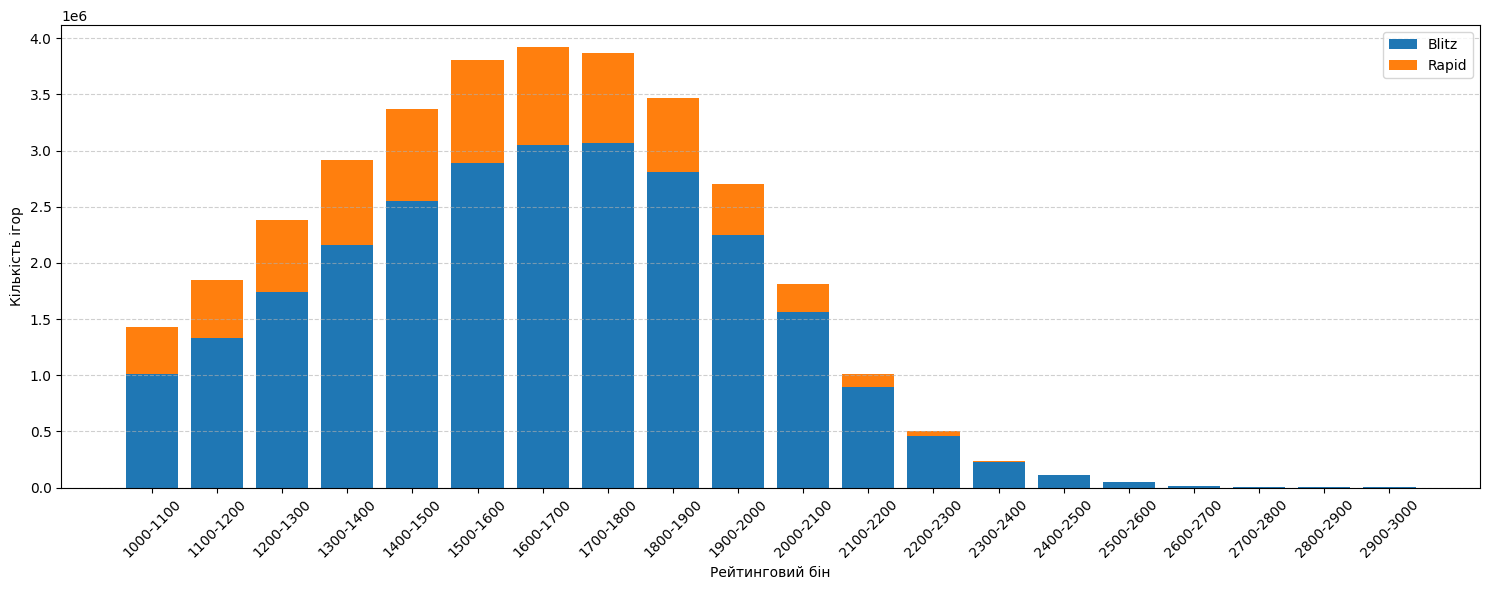
\includegraphics[width=1\textwidth]{Images/rating-distr.png}

    \vspace{4mm}
    \begin{itemize}
        \item Для навчання моделей обрано дві рейтингові групи:
        \begin{itemize}
            \item \textbf{1600--1700} — 3\,919\,708 партій;
            \item \textbf{2000+} — 3\,755\,324 партій.
        \end{itemize}
    \end{itemize}
\end{frame}

\begin{frame}[t]
    \frametitle{Валідація результатів}

    \begin{itemize}
        \item Для оцінки сили гри було проведено матч між двома моделями: 2000+ та 1600--1700.
        \item Було просимулювано 1000 партій з температурою softmax T = 0.1 для уникнення повторів.
        \item Використано ендшпільні таблиці Syzygy (3–5 фігур).
    \end{itemize}

    \vspace{2mm}
    \textbf{Результати:}
    \begin{itemize}
        \item Перемоги моделі 2000+: 677, поразки: 63, нічиї: 260.
        \item Відсоток очок: 80.8%
        \item Розрахована різниця рейтингів за формулою Ело:
        \[
        D = -400 \cdot \log_{10} \left( \frac{1}{0.808} - 1 \right) \approx 241.6
        \]
        \item Очікувана різниця: приблизно 300–400 пунктів (середнє — 350).
        \item Фактична різниця (за результатами матчу): 242 пункти.
        \item Відхилення становить близько 100 пунктів рейтингу, що, ймовірно, пов’язано з обмеженим обсягом навчальних даних і доданою температурою у softmax, яка підвищує стохастичність гри.
    \end{itemize}
\end{frame}




\begin{frame}[t]
    \frametitle{Оцінка людяності}

    \begin{itemize}
        \item Для додаткової валідації моделі перевіряємо, наскільки передбачений хід рушія збігається з фактичним ходом гравця.
        \item Це дозволяє оцінити \textbf{людяність} моделі — здатність імітувати поведінку гравців різного рівня.
        \item Для проведення оцінки було використано такі дані:
        \begin{itemize}
            \item партії з Lichess за квітень 2025 року;
            \item з ~50\,000 партій отримано 320\,000 позицій;
            \item позиції згруповано за рейтингом гравців з кроком 100 — від 1000 до 2500;
            \item відповідно для кожного рейтингового інтервалу відібрано по 20\,000 позицій.
        \end{itemize}
    \end{itemize}
\end{frame}

\begin{frame}[t]
    \frametitle{Результати оцінки людяності}
    \begin{figure}
        \centering
        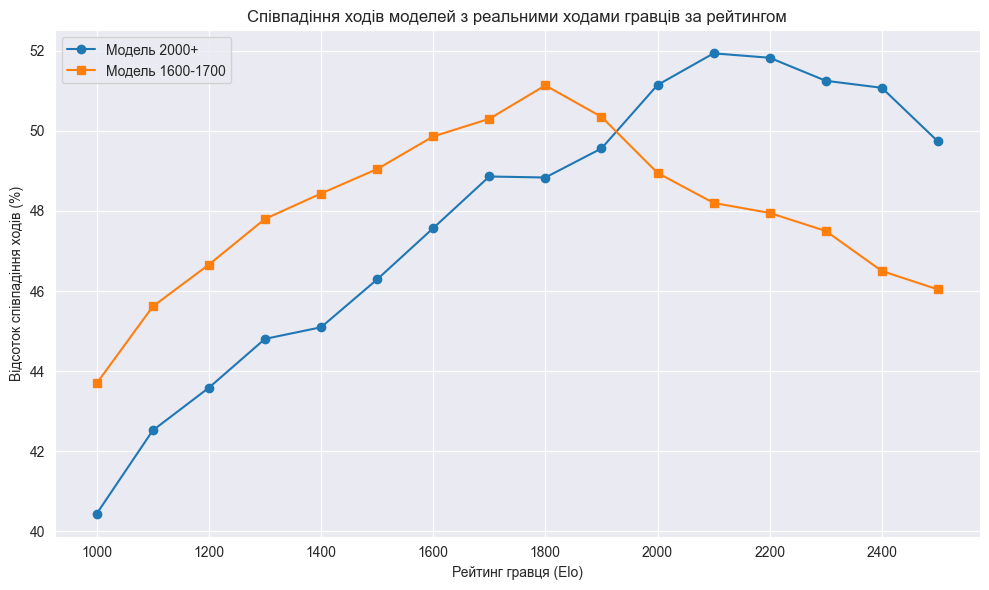
\includegraphics[width=0.75\textwidth]{Images/validation1.png}
    \end{figure}
    \begin{itemize}
        \item Модель 1600–1700 найкраще узгоджується з гравцями 1600–1900, максимум — 51.135\% на 1800.
        \item Модель 2000+ точніше відтворює ходи сильніших гравців, максимум — 51.935\% на 2100.
    \end{itemize}
\end{frame}

\begin{frame}[t]
    \frametitle{Порівняння з класичним рушієм Stockfish}

    \begin{itemize}
        \item Для оцінки сили гри моделей порівнюємо їх зі Stockfish — класичним рушієм із детермінованим пошуком.
        \item Щоб зробити порівняння коректним, обмежуємо Stockfish за глибиною пошуку (від 4 до 11).
        \item На кожній фіксованій глибині моделі грають по 1000 партій проти Stockfish.
        \item Таким чином визначаємо, яка глибина відповідає силі гри кожної моделі.
        \item Крім того, аналізуємо не лише силу, але й стиль гри — наскільки він \textbf{людяний}.
    \end{itemize}
\end{frame}

\begin{frame}[t]
    \frametitle{Результати матчів зі Stockfish}

    \begin{itemize}
        \item Проведено по 1000 партій між кожною моделлю та Stockfish на різних глибинах.
        \item Визначено орієнтовну відповідність сили гри наших моделей до глибини пошуку Stockfish.
    \end{itemize}

    \vspace{2mm}

    \begin{minipage}{0.48\textwidth}
        \centering
        {Модель 1600--1700} \\
        \scriptsize
        \begin{tabular}{|c|c|}
            \hline
            Глибина Stockfish & Очки (\%) \\
            \hline
            4 & 87.15 \\
            5 & 65.75 \\
            6 & 43.20 \\
            7 & 24.15 \\
            \hline
        \end{tabular}
    \end{minipage}
    \hfill
    \begin{minipage}{0.48\textwidth}
        \centering
        {Модель 2000+} \\
        \scriptsize
        \begin{tabular}{|c|c|}
            \hline
            Глибина Stockfish & Очки (\%) \\
            \hline
            8  & 86.20 \\
            9  & 61.60 \\
            10 & 39.50 \\
            11 & 15.85 \\
            \hline
        \end{tabular}
    \end{minipage}

    \vspace{4mm}

    \begin{itemize}
        \item Модель 1600--1700 ≈ рівень Stockfish між глибинами 5 і 6.
        \item Модель 2000+ ≈ рівень Stockfish між глибинами 9 і 10.
    \end{itemize}
\end{frame}

\begin{frame}[t]
    \frametitle{Порівняння людяності з Stockfish}
        \begin{figure}
        \centering
        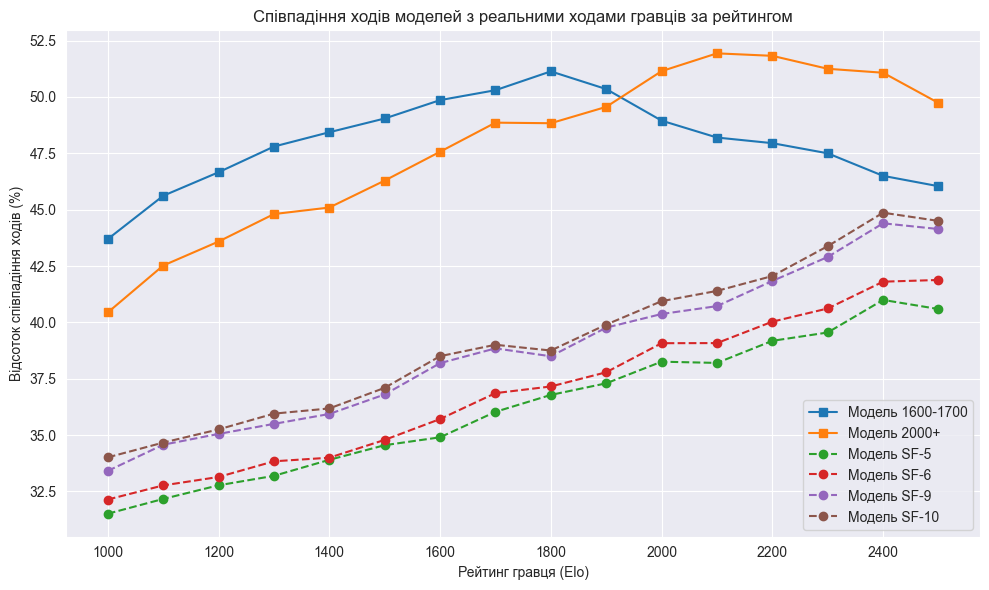
\includegraphics[width=0.65\textwidth]{Images/validation2.png}
    \end{figure}

    \begin{itemize}
        \item Stockfish не адаптує до стилю гравців, графіки не мають чітко виражених піків — точність монотонно зростає з рейтингом.
        \item Натомість наша модель демонструє вищі результати передбачення саме в цільових рейтингових групах, для яких вона була навчена.
        \item Це свідчить про наявність {людяної поведінки} — здатності імітувати типові помилки, пріоритети та стиль гри гравців конкретного рівня.
    \end{itemize}


\end{frame}

\begin{frame}[t]
    \frametitle{Графічний інтерфейс користувача}

    \begin{itemize}
        \item Користувач може:
        \begin{itemize}
            \item обрати колір фігур;
            \item встановити рівень бота (1600--1700 або 2000+);
            \item зіграти партію проти моделі;
            \item завершити гру достроково (кнопка ``Здатися'').
        \end{itemize}
    \end{itemize}

    \centering
    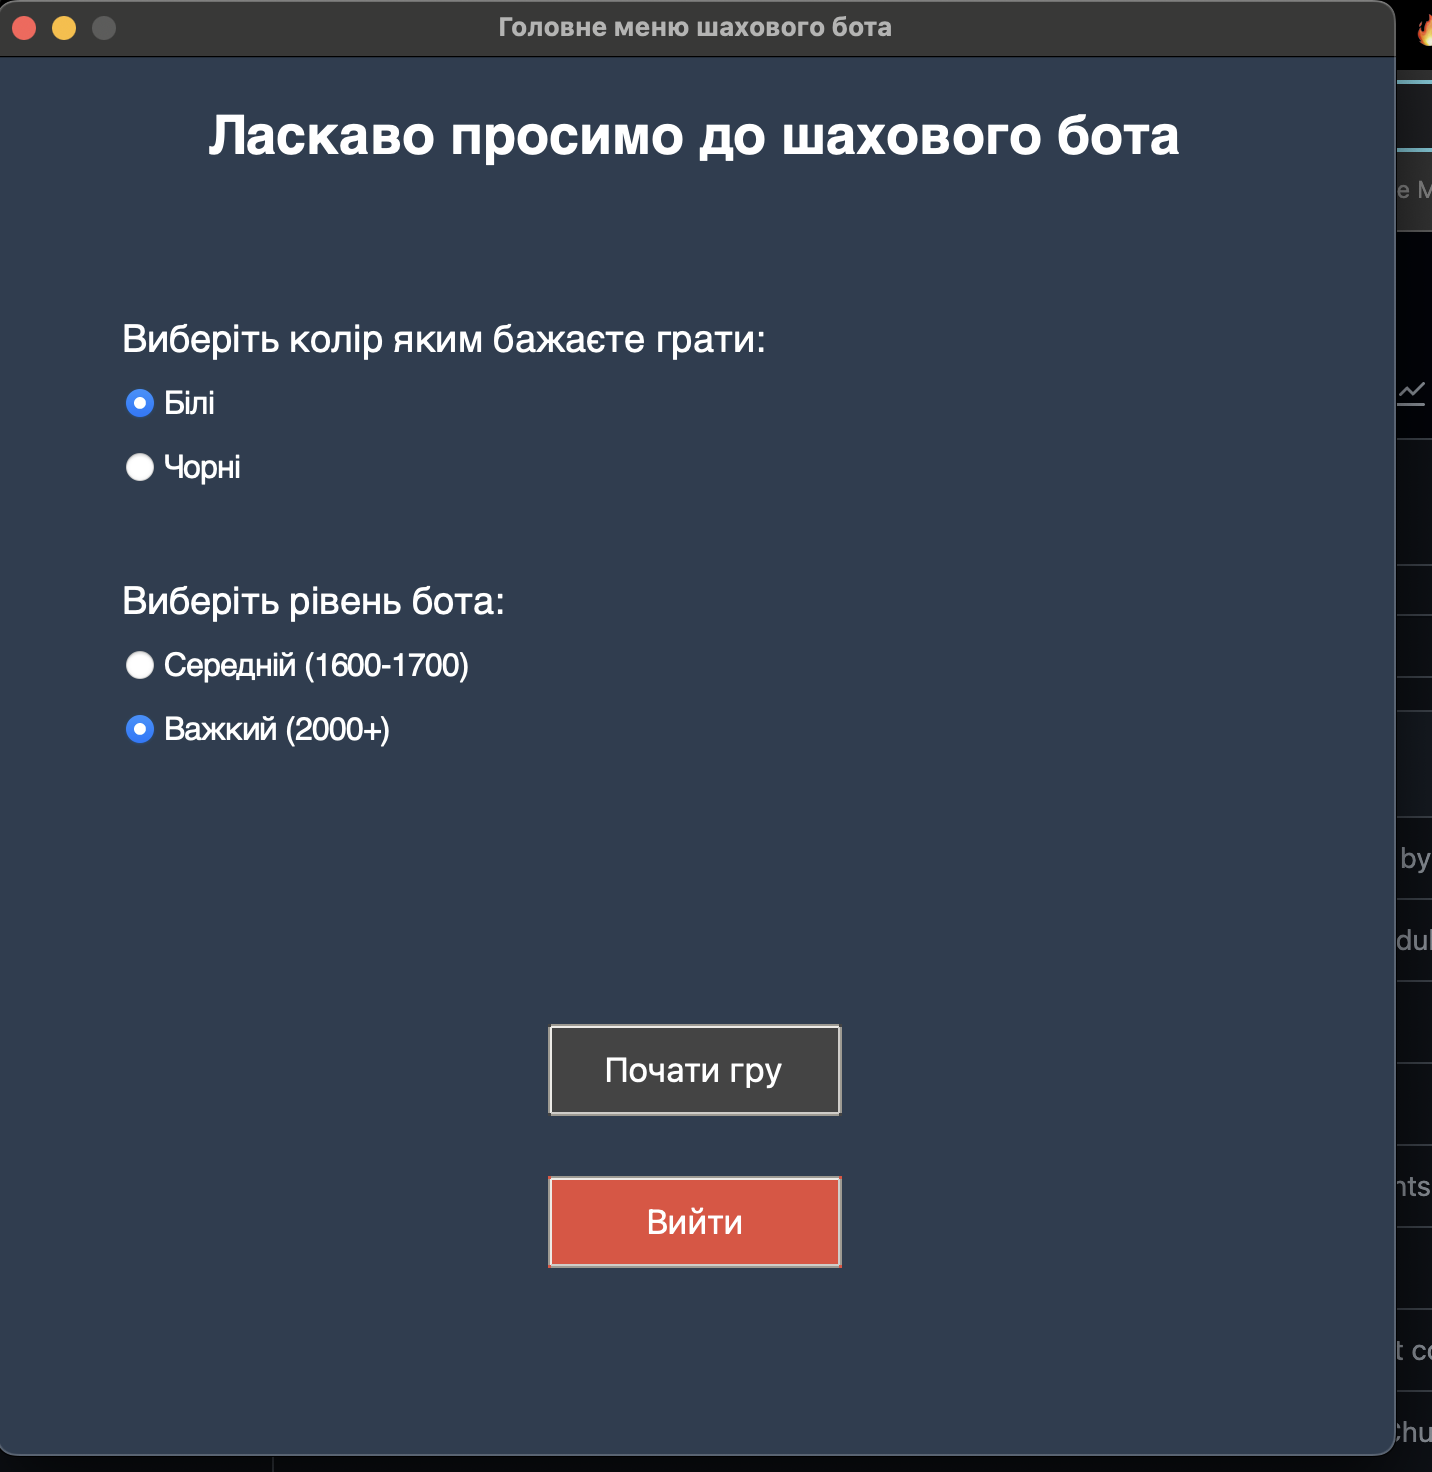
\includegraphics[width=0.4\textwidth]{Images/main-menu.png}%
    \hfill
    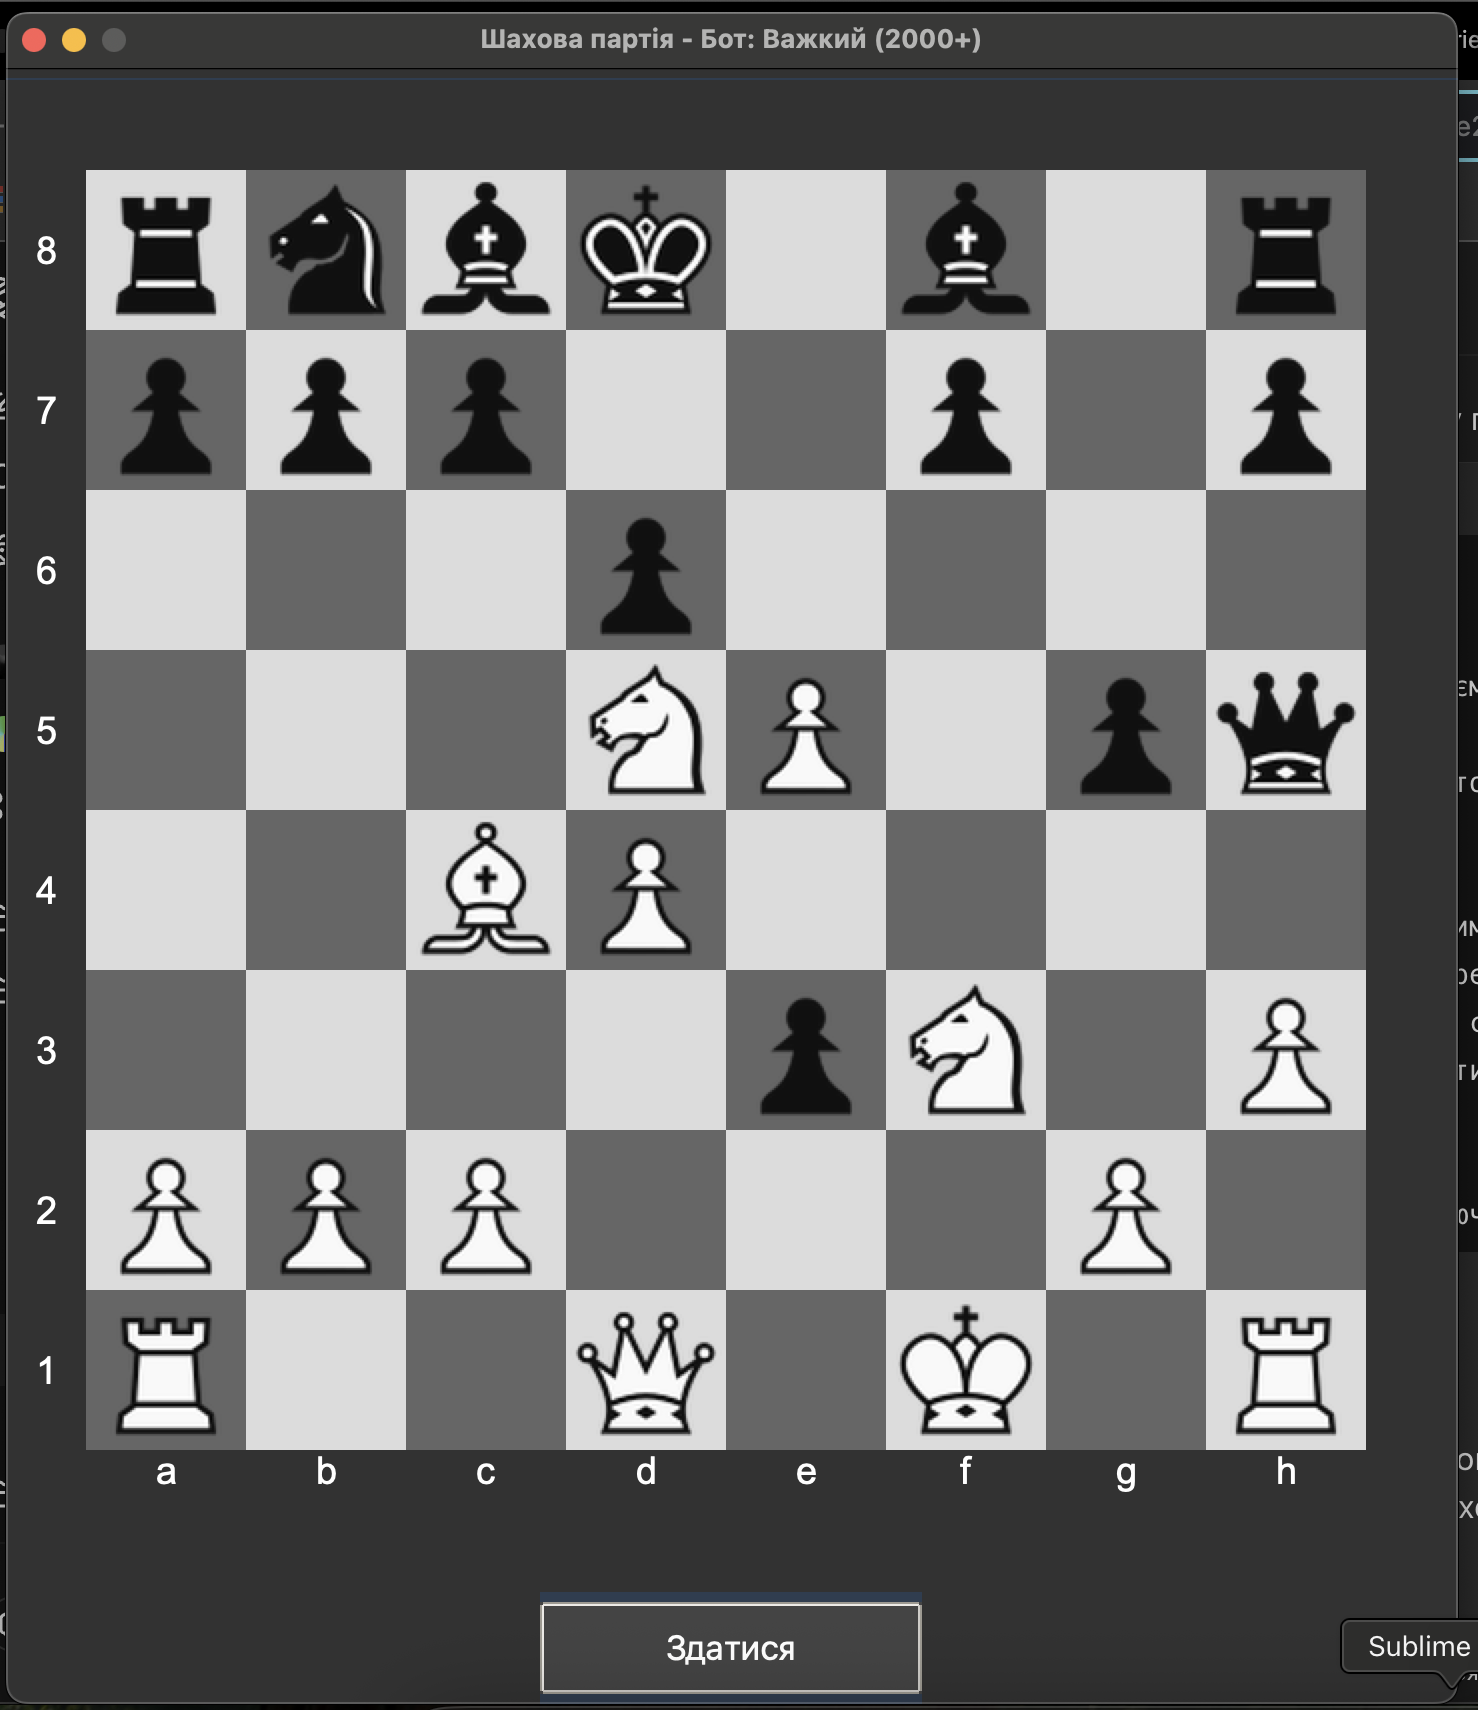
\includegraphics[width=0.4\textwidth]{Images/game-mid.png}
\end{frame}



\begin{frame}[t]
    \frametitle{Архітектура}

    \begin{columns}
        % Ліва колонка — текст
        \begin{column}{0.55\textwidth}
            \begin{itemize}
                \item Отримання PGN-партій з бази \textit{Lichess}.
                \item Препроцесинг → структуровані позиції.
                \item Навчання двох моделей (1600--1700 та 2000+).
                \item Інтеграція моделей у рушій Lc0.
                \item Розгортання GUI-додатку для гри.
            \end{itemize}
        \end{column}

        % Права колонка — діаграма
        \begin{column}{0.35\textwidth}
            \centering
            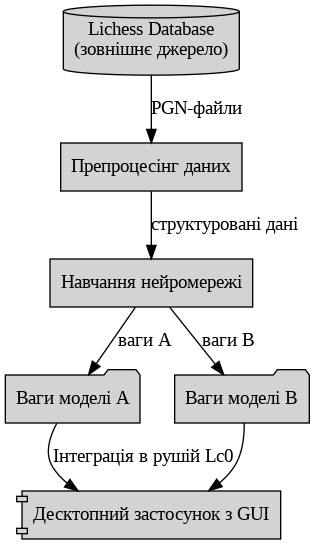
\includegraphics[width=\linewidth]{Images/system-diagram.png}
            \vspace{2mm}
        
        \end{column}
    \end{columns}
\end{frame}

\begin{frame}[t]
    \frametitle{Висновки}

    \begin{itemize}
        \item Реалізовано повний цикл побудови адаптивного шахового рушія, що імітує стиль гри людини на заданому рейтинговому рівні.
        \item Основою рушія стала згорткова нейромережа типу ResNet.
        \item Навчано дві моделі:
        \begin{itemize}
            \item рівень 1600--1700 — 3\,919\,708 партій;
            \item рівень 2000+ — 3\,755\,324 партій.
        \end{itemize}
        \item В результаті симуляційного матчу модель 2000+ здобула 80.8\% очок проти моделі 1600--1700 (≈241 пункт Ело).
        \item Порівняння зі Stockfish показало відповідність рівнів гри: 
        \begin{itemize}
            \item модель 1600--1700 — між глибинами 5 і 6;
            \item модель 2000+ — між глибинами 9 і 10.
        \end{itemize}
        \item Модель 1600--1700 досягає піку точності 51.1\% на рейтингу 1800, модель 2000+ — 51.9\% на 2100, що на 10--15\%  більше, ніж у відповідних моделей Stockfish на тих самих таргетованих рейтингах.
    \end{itemize}
\end{frame}




\end{document}
